 % Pacotes e configurações padrão do estilo "article"\
% -------------------------------------
\documentclass[a4paper,twocolumn,11pt]{article}
%\documentclass[a4paper,11pt]{article} 
% Layout
% --------------------------------------------------------------------------------
%     Gráficos e layout ----------------------------------------------------------------------

\ifx\pdfmatch\undefined
\else
    \usepackage[T1]{fontenc}
    \usepackage[utf8]{inputenc}
\fi
% xetex:
\ifx\XeTeXinterchartoks\undefined
\else
    \usepackage{fontspec}
    \defaultfontfeatures{Ligatures=TeX}
\fi
% luatex:
\ifx\directlua\undefined
\else
    \usepackage{fontspec}
\fi
% End engine-specific settings

%      Fonte --------------------------------------------------------------------------------
%\usepackage{lmodern}
\usepackage{times}
%     Pacotes adicionados -------------------------------------------------------------------
\usepackage{ae}
%     Língua e hifenização ------------------------------------------------------------------
\usepackage[english]{babel}
\usepackage{hyphenat}
%      Outros --------------------------------------------------------------------------------
\usepackage{fancyhdr}
\usepackage{sectsty}
\usepackage{float}
%\usepackage{graphicx}
\usepackage[pdftex]{color,graphicx}
\usepackage{hyperref}
\usepackage{enumerate} % Permite alterar Layout do enumerate
%\usepackage{pdflscape} % Permite alterar a orientação da pagina
%\usepackage{ifthen} % Permite usar condicionais ifelse
%\usepackage[table]{xcolor} % Permite alterar as cores das celulas de uma tabela
\usepackage{amsmath,amssymb} % Ambiente para uso de elementos matemáticos
\usepackage{caption}
\usepackage{subcaption} % permite o uso de multiplas figuras com legenda
%\usepackage{minted} % FOrmatador para códigos de programas
% Layout do documento ------------------------------------------------------------------------
%     Bordas e tamanho da página ------------------------------------------------------------
\usepackage{geometry} 
 \geometry{ % Padrâo ABNT para relatórios
 a4paper,
 left=30mm,
 right=20mm,
 top=30mm,
 bottom=20mm
 }
%     Cabeçalho e Rodapé ---------------------------------------------------------------
\pagestyle{fancy}
  \lhead{}
  \chead{}
  \rhead{}
  \lfoot{}
  \cfoot{}
  \rfoot{\thepage}
%     Númeração ------------------------------------------------------------------------
  \pagenumbering{arabic}
%     Retas do cabeçalho e rodapé ------------------------------------------------------
  \renewcommand{\headrulewidth}{0.5pt}
  \renewcommand{\footrulewidth}{0.5pt}
%     Tamanho da letra de seções e derivadas --------------------------------------------
  \sectionfont{\normalsize}
  \subsectionfont{\small}
%     Hiperlinks ------------------------------------------------------------------------
  \hypersetup{
                  colorlinks,
                  citecolor=black,
                  filecolor=black,
                  linkcolor=black,
                  urlcolor=black
                  }
%     Dados do título e autores --------------------------------------------------------------
%\title{\tituloRelatorio}
\author{Rafael Lima}
%     Definições do pdf ----------------------------------------------------------------------
\hypersetup{
    unicode=false,          % non-Latin characters in Acrobat’s bookmarks
    pdftoolbar=true,        % show Acrobat’s toolbar?
    pdfmenubar=true,        % show Acrobat’s menu?
    pdffitwindow=false,     % window fit to page when opened
    pdfstartview={FitH},    % fits the width of the page to the window    
    pdfauthor={Rafael Lima},     % author
    pdfnewwindow=true      % links in new window
}
%     Outros ----------------------------------------------------------------------------
      %\renewcommand{\thesection}{(\alph{section})} % muda o estilo de númeração das sections
      % alterando a formatação dos numeradores de lista de itens
      \renewcommand\theenumi{\arabic{enumi}}
      \renewcommand\labelenumi{(\textit{\theenumi})}
    \renewcommand\theenumii{\arabic{enumii}}
    \renewcommand\labelenumii{(\textit{\theenumi.\theenumii})}
      
% ---------------------------------------------------------------------------------------


\usepackage[makestderr]{pythontex}
%\restartpythontexsession{\thesection}

\newcommand{\tituloRelatorio}{Transporte de Calor e Massa\\Lista 2}
\title{\tituloRelatorio}
\hypersetup{pdftitle={\tituloRelatorio}}% title

% Definições Auxiliares
% -----------------------------------------------------------------
%\input{relat_aux.tex}
\renewcommand{\thesection}{Questão \arabic{section}:} 
\renewcommand{\thesubsection}{(\alph{subsection})}
\newcommand{\npy}[1]{\sympy{round(n#1,4)}}
\newcommand{\epy}[1]{\sympy{#1} = \sympy{s#1}}
\newcommand{\nnpy}[1]{\sympy{#1} = \sympy{round(n#1,4)}}
% ----------------------------------~>ø<~---------------------------------------
\begin{document}
% Capa e Índice ---------------------------------------------------------------
\maketitle
% Conteudo -------------------------------------------------------------------
\section{} % q1
\begin{figure}[H]
\centering
\includegraphics[width = 0.9\linewidth]{./image/lista2/q1}
\end{figure}

\begin{sympycode}
# Symbolic
Pa = Symbol('P_atm') # Pressão Atmosférica
Pp = Symbol('P_p') # Pressão Exercida pelo Peso do Pistão
Pm = Symbol('P_m') # Pressão Exercida pela Mola
Fm = Symbol('F_m') # Força Exercida pela Mola
A = Symbol('A') # Área Pistão
mp = Symbol('m_p') # Massa Pistão
g = Symbol('g') # Constante Gravidade

sPm = Fm/A
sPp = (mp*g)/A
P = Pa + Pm +Pp

# Numeric
nPa = 95e3 # Pa
nFm = 60 # N
nmp = 4 # kg
ng = 9.81 # kg*m/s^2
nA = 35/(100**2) # m^2

nPm = nFm/nA
nPp = (nmp*ng)/nA
nP = nPa + nPm +nPp
\end{sympycode}

A pressão total dentro do cilindro $P$ será dada pela soma da pressão atmosférica $\sympy{Pa}$, mais a pressão exercida pela mola $\sympy{Pm}$ e da exercida pelo peso do pistão $\sympy{Pp}$. Dado que pressão exercída pela mola é $\epy{Pm}= \npy{Pm/1000}\ kPa$ , a pressão exercida pelo peso do pistão é $\epy{Pp}= \npy{Pp/1000}\ kPa$ e a presão atmosférica é $\sympy{Pa} = \npy{Pa/1000}\ kPa$, temos $P = \sympy{P} = \npy{Pa} + \npy{Pp} + \npy{Pm}$ e portanto: $P = \npy{P} = \npy{P/1000}\ kPa$

\section{} % q2
\begin{sympycode}
# Symbolic
Pa = Symbol('P_atm') # Pressão Atmosférica
Pc = Symbol('P_c') # Pressão Manometro
h = Symbol('h') # Altura Coluna
g = Symbol('g') # Constante Gravidade
p = Symbol('rho_m') # Densidade Mercúrio

# Numeric
nPa = 100e3 # Pa
nh = 10e-3 # m
np = 13600 # kg/m^3

dP = p*h
ndP = np*nh
nPc = ndP + nPa

\end{sympycode}
\begin{figure}[ht]
\centering
\label{fig:l2q2}
\includegraphics[width = 0.9\linewidth]{./image/lista2/q2}
\caption{Manômetro a mercúrio}
\end{figure}

\subsection{}\label{q2a} Com base na figura \ref{fig:l2q2}, percebe-se que a pressão exercída pelo duto de ar é maior que a pressão atmosférica.
\subsection{} Podemos verificar e fenomeno observado no item \ref{q2a} tomando dois pontos na mesma altura, um na inteface entre o mercúrio e o duto de ar e outro no meio da coluna de mercúrio. Desta forma temos que a pressão no tubo será dado por $\sympy{Pc} = \sympy{dP} + \sympy{Pa}$ e portanto $\sympy{Pc} = \npy{dP/1000} + \npy{Pa/1000} = \npy{Pc/1000}\ kPa$

\section{} % q3
\begin{sympycode}
# Symbolic
F1 = Symbol('F_1') # Força peso
F2 = Symbol('F_1') # Força peso fluído
p = Symbol('rho') # densidade fluido
A1 = Symbol('A_1') # Área cilindro 1
A2 = Symbol('A_2') # Área cilindro 2
h = Symbol('h') # altura coluna
m = Symbol('m') # Massa
g = Symbol('g') # constante Gravidade

sF2 = F1*(A2/A1)
sF1 = m*g
sh = sF1/(A1*p)

np = 780
nm = 500
ng = 9.81
nd1 = 1.2
nA1 = nd1*nd1*pi/4
nh = nm/(np*nA1)
\end{sympycode}
A partir do princípio de Pascal temos $$\sympy{F1/A1} = \sympy{F2/A2}$$
Como a variação de pressão na coluna é $P = \sympy{F2/A2} = \sympy{p*h}$ e que $\epy{F1}$, então
$$\sympy{F1/A1} = \sympy{(m*g)/A1} = \sympy{p*h*g}$$
Dividindo por $g$ e isolando $h$ temos
$$
h = \sympy{sh} = \npy{h}\ m
$$

\section{} % q4
\begin{sympycode}
# Symbolic
Pa = Symbol('P_atm') # Pressão Atmosférica
P0 = Symbol('P_c') # Pressão Balão
h1 = Symbol('h_1') # Altura Coluna 1
h2 = Symbol('h_2') # Altura Coluna 1
g = Symbol('g') # Constante Gravidade
g1 = Symbol('g_1') # Gravidade Especifica Fluído 1
g2 = Symbol('g_2') # Gravidade Especifica Fluído 2
p1 = Symbol('rho_1') # Densidade Fluido 1
p2 = Symbol('rho_2') # Densidade Fluido 2
pa = Symbol('rho_a') # Densidade Água

sg1 = p1/pa
sg2 = p2/pa

sp2 = p1*(h1/h2) - (Pa-P0)/(h2*g)
sg22 = (p1/pa)*(h1/h2) - (Pa-P0)/(h2*g*pa)
sg23 = g1*(h1/h2) - (Pa-P0)/(h2*g*pa)

# Numeric
nPa = 100e3 # Pa
nP0 = 76e3 # Pa
nh1 = 22e-2 # m
nh2 = 40e-2 # m
np1 = 13550 # kg/m^3
ng1 = 13.55
npa = 1000 # kg/m^3
ng = 9.81 # kg*m/s^2

ng2 = sg22.subs([[Pa,nPa],[P0,nP0],\
    [h1,nh1],[h2,nh2],[p1,np1],[pa,npa],[g,ng]])

\end{sympycode}

\begin{figure}[H]
\centering
\label{fig:l2q4}
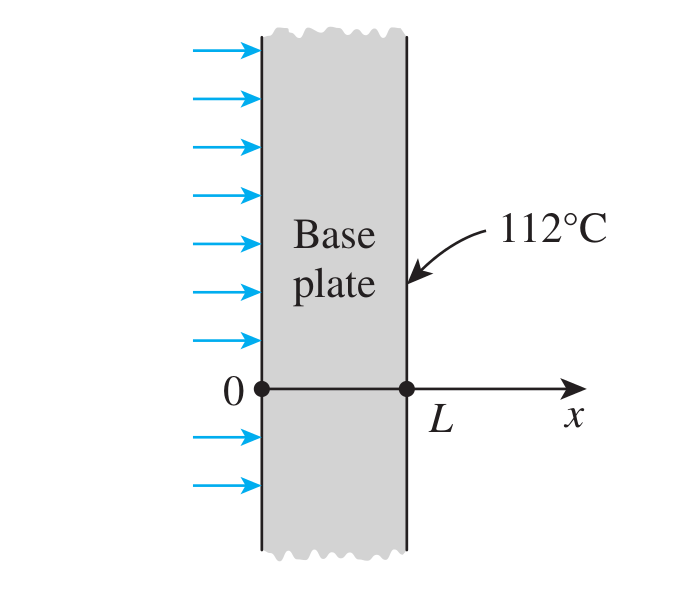
\includegraphics[width = 0.9\linewidth]{./image/lista2/q4}
\caption{Manômetro com duplo fluído}
\end{figure}

Tomando um ponto em cada lado do manômetro na altura aonde ocorre a interface entre os dois flúidos temos:
\begin{equation}\label{eq:l2q4-1}
\sympy{P0 + p1*h1*g} = \sympy{Pa + p2*h2*g}
\end{equation}
Isolando $\sympy{p2}$ em \eqref{eq:l2q4-1} temos:
$$
\sympy{p2}=\sympy{sp2}
$$
Dividindo pela densidade da água:
$$
\sympy{p2/pa}=\sympy{(p1/pa)*(h1/h2) - (Pa-P0)/(h2*g*pa)}
$$
Dado que $\epy{g1}$ e $\epy{g2}$, substituindo em 
\begin{equation}\label{eq:l2q4-2}
\sympy{g2}=\sympy{sg23}% = (\npy{g1})\cdot\frac{\npy{h1}}{\npy{h2}} + \frac{\s}
\end{equation}
Substituindo os valores de $\nnpy{g1}$ , $\nnpy{Pa}\ Pa$ , $\nnpy{P0} Pa$ , $\nnpy{h1} m$ , $\nnpy{h2} m$ , $\nnpy{g} Kg m/s^2$ e $\nnpy{pa}\ Kg/m^3$ na equação \eqref{eq:l2q4-2} temos que $\nnpy{g2}$.

\section{} % q5

\begin{sympycode}
# Symbolic
Pa = Symbol('P_A') # Pressão em A
Pb = Symbol('P_B') # Pressão em B
Pn = Symbol('P_m') # Pressão em M
Pg = Symbol('P_g') # Pressão em G
P1 = Symbol('P_1') # Pressão em 1
P2 = Symbol('P_2') # Pressão em 2
ha = Symbol('h_A') # Altura Coluna 1
hb = Symbol('h_B') # Altura Coluna 1
hm = Symbol('h_m') # Altura Coluna 1
hg = Symbol('h_g') # Altura Coluna 1

g = Symbol('g') # Constante Gravidade
pa = Symbol('rho_A') # Densidade A
pb = Symbol('rho_B') # Densidade B
pm = Symbol('rho_m') # Densidade A
pg = Symbol('rho_g') # Densidade A
paq = Symbol('rho_a') # Densidade A

ga = Symbol('SG_A') # Gravidade Especifica
gb = Symbol('SG_B') # Gravidade Especifica
gm = Symbol('SG_m') # Gravidade Especifica
gg = Symbol('SG_g') # Gravidade Especifica

sP2 = Pa - pa*ha*g - pm*hm*g
sP1 = P2 + pg*hg*g
sPb = P1 - pb*hb*g
sPab  = g*(pa*ha + pm*hm - pg*hg + pb*hb)
sPab2  = g*(ga*ha + gm*hm - gg*hg + gb*hb)

nga = 1
ngb = 0.88
ngm = 13.5
ngg = 1.26
ng = 9.81

nha = 55e-2
nhm = 20e-2
nhg = 20e-2 + 12e-2 + 10e-2
nhb = 10e-2

nPab2  = ng*(nga*nha + ngm*nhm - ngg*nhg + ngb*nhb)

\end{sympycode}
\begin{figure}[H]
\centering
\label{fig:l2q5}
\includegraphics[width = 0.9\linewidth]{./image/lista2/q5}
\caption{Manômetro com duplo fluído}
\end{figure}

Tomando dois pontos de referência de pressão $P_1$ e $P_2$ temos
$$
\left\{
\begin{array}{l}
\epy{P2}\\
\epy{P1}\\
\epy{Pb}\\
\end{array}
\right.
$$

Resolvendo o sistema e isolando $\sympy{Pa-Pb}$ temos
\begin{equation}
\sympy{Pa-Pb} = \sympy{sPab}
\end{equation}
Dividindo tudo pela densidade da água $\sympy{paq}$
$$
\sympy{(Pa-Pb)/paq} = \sympy{sPab/paq}
$$
Logo podemos calcular $\sympy{(Pa-Pb)}$ como 
\begin{equation}
\sympy{(Pa-Pb)} = \sympy{sPab2}
\end{equation}
Portanto o valor da diferênça de pressão é $\sympy{(Pa-Pb)} = \npy{Pab2}\ kPa$.

\section{} % q6
\begin{sympycode}
# Symbolic
Pa = Symbol('P_atm') # Pressão em A
P0 = Symbol('P_0') # Pressão em B
P1 = Symbol('P_1') # Pressão em 1
P2 = Symbol('P_2') # Pressão em 2
ha = Symbol('h_A') # Altura Coluna A
hm = Symbol('h_m') # Altura Coluna h
h0 = Symbol('h_0') # Altura Coluna B
g = Symbol('g') # Constante Gravidade
pa = Symbol('rho_A') # Densidade A
p0 = Symbol('rho_0') # Densidade B
pm = Symbol('rho_m') # Densidade A
paq = Symbol('rho_a') # Densidade A
ga = Symbol('SG_A') # Gravidade Especifica
g0 = Symbol('SG_0') # Gravidade Especifica
gm = Symbol('SG_m') # Gravidade Especifica

sP1 = P0 + paq*ha*g
sP2 = Pa + g*(p0*h0 + pm*hm)

shm  = (P0 - Pa)/(paq*gm*g) + (-ga*ha + g0*h0)/(gm)
shm.simplify()

nga = 1
ng0 = 0.72
ngm = 13.5
npaq = 1000

nP0 = 65e3
nPa = 0e3

nha = 30e-2
nh0 = 75e-2

nhm = shm.subs([[P0,nP0],[Pa,nPa],[g0,ng0],[paq,npaq],\
    [gm,ngm],[h0,nh0],[ha,nha],[ga,nga]])
\end{sympycode}


\begin{figure}[H]
\centering
\label{fig:l2q6}
\includegraphics[width = 0.9\linewidth]{./image/lista2/q6}
\caption{}
\end{figure}

\begin{equation}\label{eq:l2q6-1}
\left\{
\begin{array}{l}
\sympy{sP1} = P_1\\
\sympy{sP2} = P_1\\
\end{array}
\right.
\end{equation}
Subtraindo as duas expressões em \eqref{eq:l2q6-1} temos
$$\sympy{sP2-sP1} = 0$$
\begin{equation}\label{eq:l2q6-2}
hm = \sympy{(Pb-Pa)/(pm*2*g)}
\end{equation}

\begin{equation}
\sympy{shm}
\end{equation}

\section{Manômetro de Tubos Inclinados} % q7
\begin{sympycode}
# Symbolic
Pa = Symbol('P_A') # Pressão em A
Pb = Symbol('P_B') # Pressão em B
P0 = Symbol('P_0') # Pressão em 1
ha = Symbol('h_A') # Altura Coluna A
hm = Symbol('h_m') # Altura Coluna h

g = Symbol('g') # Constante Gravidade
a = Symbol('a')
angle = Symbol('theta')
paq = Symbol('rho_a') # Densidade A
pb = Symbol('rho_a') # Densidade B
pm = Symbol('rho_m') # Densidade A

ga = Symbol('SG_a') # Gravidade Especifica
gm = Symbol('SG_m') # Gravidade Especifica

sP1 = Pa+paq*a*g+pm*2*a*g
sP2 = Pb+paq*a*g

sa = (Pb - Pa)/(paq*gm*2*g)

# Numeric
nl = 0.268 # m
ng = 9.81  # m/s^2
ngm = 13.5
npaq = 1000

nPb = 20e3
nPa = 0e3

na = sa.subs([[Pb,nPb],[Pa,nPa],[g,ng],[paq,npaq],[gm,ngm]])
\end{sympycode}

\begin{figure}[H]
\centering
\label{fig:l2q7}
\includegraphics[width = 0.9\linewidth]{./image/lista2/q7}
\caption{Manômetro com tubos inclinados}
\end{figure}

\begin{equation}\label{eq:l2q7-1}
\left\{
\begin{array}{l}
\sympy{sP1} = P_0\\
\sympy{sP2} = P_0\\
\end{array}
\right.
\end{equation}
Subtraindo as duas expressões em \eqref{eq:l2q18-1} temos
$$\sympy{sP2-sP1} = 0$$
\begin{equation}\label{eq:l2q7-2}
a = \sympy{(Pb-Pa)/(pm*2*g)}
\end{equation}
Subsitituindo $\sympy{pm} = \sympy{gm*paq}$ em \eqref{eq:l2q7-2}
$$
a = \sympy{(Pb-Pa)/(paq*gm*2*g)} = \frac{\npy{Pb-nPa}}{2\cdot\npy{gm}\cdot\npy{paq}}
$$
\begin{equation}\label{eq:l2q18-3}
a = \npy{a*100}\cdot 10^{-2}\ m = \npy{a*100}\ cm
\end{equation}

\section{Pressão Manométrica} % q8
\begin{sympycode}
# Symbolic
Pa = Symbol('P_atm') # Pressão em A
Pb = Symbol('P_B') # Pressão em B
P0 = Symbol('P_0') # Pressão em 0
P1 = Symbol('P_1') # Pressão em 1
P2 = Symbol('P_2') # Pressão em 2
P3 = Symbol('P_3') # Pressão em 3
ha = Symbol('h_1') # Altura Coluna A
hm = Symbol('h_3') # Altura Coluna 
ho = Symbol('h_2') # Altura Coluna B
g = Symbol('g') # Constante Gravidade
pa = Symbol('rho_A') # Densidade A
po = Symbol('rho_0') # Densidade B
pm = Symbol('rho_m') # Densidade A

P = g*(pm*hm-pa*ha-po*ho)

ng = 9.81

nha = 0.4
nho = 0.6
nhm = 0.8

npa = 1000
npo = 850
npm = 13600

nP = ng*(npm*nhm-npa*nha-npo*nho)
\end{sympycode}

\begin{figure}[H]
\centering
\label{fig:l2q8}
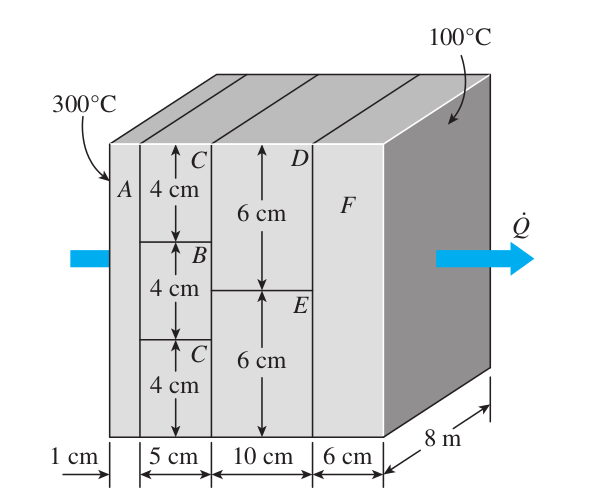
\includegraphics[width = 0.9\linewidth]{./image/lista2/q8}
\caption{Tanque}
\end{figure}

\begin{equation}\label{eq:l2q8-1}
\left\{
\begin{array}{l}
\sympy{Pa + pm*hm*g} = P_0\\
\sympy{P1 + p0*ho*g} = P_0\\
\sympy{Pb + pa*ha*g} = P_1
\end{array}
\right.
\end{equation}

Substituindo $P_1$

$$
\left\{
\begin{array}{l}
\sympy{Pa + pm*hm*g} = P_0\\
\sympy{Pb + pa*ha*g + p0*ho*g} = P_0\\
\end{array}
\right.
$$
Igualando as duas expressões:
$$
\sympy{Pb + pa*ha*g + p0*ho*g} = \sympy{Pa + pm*hm*g}
$$
Isolando $\sympy{Pb-Pa}$
\begin{equation}
\sympy{Pb -Pa} = \sympy{g*(pm*hm-pa*ha-po*ho)}
\end{equation}

Substituindo os valores das densidades $\nnpy{pm}\ kg/m^3$ , $\nnpy{pa}\ kg/m^3$ , $\nnpy{po}\ kg/m^3$ , da altura das colunas $\nnpy{ha}\ m$ , $\nnpy{hm}\ m$ , $\nnpy{ho}\ m$ e de $\nnpy{g}\ m/s^2$, a pressão manométrica será $\sympy{Pb -Pa} = \npy{P/1000}\ kPa$.

\section{Sonda} % q9
\begin{figure}[H]
\centering
\label{fig:l2q9}
\includegraphics[width = 0.9\linewidth]{./image/lista2/q9}
\caption{Sonda}
\end{figure}

A medida da pressão e da temperatura em função do tempo através da sonda mostrada na figura \ref{fig:l2q9} segue a descrição euclidiana pois leva em consideração apenas o estado do fluído no local de interesse, no caso a ponta da sonda, em relação ao tempo analisado. Esta análise se assemelha a análise de volume de controle, sendo observado o comportamento do flúido mediante a entrada e saída do fluxo do escoamento do flúido em relação a região observada.

\section{Escoamento em Duto} % q10

% Equação de Navier-Stokes 
% Mostre que o campo de velocidades é incompreensível
O escoamento será incompressível pois $\nabla \vec{V} = 0$ pois
$$\nabla \vec{V} = \frac{\delta \vec{V_x}}{\delta x} + \frac{\delta \vec{V_y}}{\delta y}$$
$$\nabla \vec{V} = \frac{\delta (U_0+b x))}{\delta x} + \frac{\delta (-b y)}{\delta t}$$
$\nabla \vec{V} = b - b = 0$

\begin{equation}
\vec{a} = \frac{d_m \vec{V}}{dt} = \frac{d \vec{V}}{dt} + (\nabla\cdot\vec{V})\cdot\vec{V}
\end{equation}
Como $\frac{d \vec{V}}{dt} = 0$ pois não depende do tempo:
$$
\vec{a} = (\nabla\cdot\vec{V})\cdot\vec{V}
$$
$$
\vec{a} = b(U_0 + b x) i + b^2
$$

\section{} % q11
O escoamento será incompressível pois $\nabla \vec{V} = 0$ pois
$$\nabla \vec{V} = \frac{\delta \vec{V_x}}{\delta x} + \frac{\delta \vec{V_y}}{\delta y}$$
$$\nabla \vec{V} = \frac{\delta (1.1+2.8x+0.65y)}{\delta x} + \frac{\delta (0.98 -2.1x - 2.8y)}{\delta t}$$
$\nabla \vec{V} = 2.8 - 2.8 = 0$
O campo de aceleração será
$$
\vec{a} = (\nabla\cdot\vec{V})\cdot\vec{V}
$$
$$
\vec{a_x(x,y)} = 2.8 (1.1+2.8x+0.65y)
$$
$$
\vec{a_y(x,y)} = -2.8 (0.98 -2.1x - 2.8y)
$$
Portanto  $\vec{a}(-2,3) = (-9,2;14.37)$
\section{} % q12
\section{} % q13
\section{} % q14
\section{} % q15
\section{} % q16
A vazão volumétrica é a medida da quantidade de volume de escoamento por unidade de tempo, equannto a vazão mássica é a medida da quantidade de massa que passa por uma seção por unidade tempo. Podemos relacionar o volume de saída com a massa de saída a partir da densidade. Para um escoamento unidirecional, sendo a vazão volumétrica , $Q_m$ a vazão mássica, temos:$Q_v = \frac{d V}{dt}\ ,\ Q_m = \frac{d M}{dt}$. Dado que $M = V \rho $ onde $\rho$ é a densidade de fluído, podemos reescrever $Q_m$ como $Q_m = \frac{d (V \rho)}{dt}$. Considerando um fluído incomepreensível e portanto com densidade constante temos:
$$Q_m = \rho \frac{d (V)}{dt} = \rho\cdot Q_v$$. Assim a vazão mássica será igual ao produto da densidade pela vazão volumétrica.
\section{} % q17
Dado o campo vectorial definido $\vec{G}$ como:
$$\vec{G} = 2xy + \frac{1}{2}x^2 - z^2$$
O rotacional de $\vec{G}$ será definido como:
$$\nabla \vec{G} = \frac{\delta (2xy)}{\delta x} + \frac{\delta \left(\frac{1}{2}x^2\right)}{\delta y} + \frac{\delta (-z^2)}{\delta z}$$
$$\nabla \vec{G} = (2z) + (0) + (-2z) = 0$$

\section{} % q18
\begin{equation}\label{eq:l2q18-1}
\vec{\nabla} \cdot (f \vec{G}) =  \vec{G} \cdot \nabla f +  f \vec{\nabla} \cdot \vec{G}
\end{equation}
Calculando $\nabla f \cdot \vec{G}$:
$$
\nabla f =  \frac{\delta f}{\delta x} + \frac{\delta f}{\delta y} + \frac{\delta f}{\delta z}
$$
\begin{equation}\label{eq:l2q18-2}
\nabla f \cdot \vec{G} =  \frac{\delta f}{\delta x}G_x + \frac{\delta f}{\delta y}G_y + \frac{\delta f}{\delta z}G_z
\end{equation}

Calculando $\vec{\nabla} \cdot \vec{G}$:
\begin{equation}\label{eq:l2q18-3}
\vec{\nabla} \cdot \vec{G}=\frac{\delta G_x}{\delta x} + \frac{\delta G_y}{\delta y} + \frac{\delta G_z}{\delta z}
\end{equation}

Calculando $\vec{\nabla} \cdot (f \vec{G})$
$$
f\vec{G} = (f G_x,f G_y,f G_z)
$$
$$
\vec{\nabla} \cdot (f \vec{G}) = \frac{\delta (f G_x)}{\delta x} + \frac{\delta (f G_y)}{\delta y} + \frac{\delta (f G_z)}{\delta z}
$$
\begin{multline}\label{eq:l2q18-4}
\vec{\nabla} \cdot (f \vec{G}) =  \frac{\delta f}{\delta x}G_x + \frac{\delta f}{\delta y}G_y + \frac{\delta f}{\delta z}G_z\\ + f\left( \frac{\delta G_x}{\delta x} + \frac{\delta G_y}{\delta y} + \frac{\delta G_z}{\delta z} \right)
\end{multline}

Substituindo \eqref{eq:l2q18-2} e \eqref{eq:l2q18-3} em \eqref{eq:l2q18-1} o que equivale a expressão \eqref{eq:l2q18-4}.

\section{Tanque Cilíndrico} % q19
\begin{sympycode}
Q1,Q2,Q3 = symbols('Q_1 Q_2 Q_3')
A1,A2 = symbols('A_1 A_2')
V1,V2 = symbols('V_1 V_2')
d1,d2,d0 = symbols('D_1 D_2 D_0')
M = Symbol('M')
t = Symbol('t')
h = Symbol('h')

dh = (Q1+Q2+Q3)/(d0**2*pi/4)

sQ1 = V1*d1**2*pi/4
sQ2 = V2*d2**2*pi/4

sV2 = V1*(d1/d2)**2 + 4*Q3/(pi*d2**2)
\end{sympycode}
\subsection{}
Relacionando a altura $h$ com o volume do tanque $M$, a varição do volume de água será dada por
\begin{equation}\label{eq:l2q19-1}
\frac{d M}{dt} = \frac{d}{dt}\sympy{(h * d0**2*pi/4)} = \sympy{(d0**2*pi/4)}\frac{d h}{dt}
\end{equation}
Assumindo o escoamento como incompreensível a vazão total do tanque será
\begin{equation}\label{eq:l2q19-2}
\frac{d M}{dt} = \sympy{Q1+Q2+Q3}
\end{equation}
Combinando as equações \eqref{eq:l2q19-1} e \eqref{eq:l2q19-2}
$$\sympy{Q1+Q2+Q3} = \sympy{(d0**2*pi/4)}\frac{d h}{dt}$$
\begin{equation}
\frac{d h}{dt} = \sympy{(Q1+Q2+Q3)/(d0**2*pi/4)}
\end{equation}

\subsection{}
Assumindo $\frac{d h}{dt} = 0$.
$$0 = \sympy{(Q1+Q2+Q3)/(d0**2*pi/4)}$$
$$\sympy{Q1+Q3} = \sympy{Q2}$$
Sabendo-se que $\epy{Q1}$ e $\epy{Q2}$
$$\sympy{sQ1+Q3} = \sympy{sQ2}$$
Isolando $\sympy{V2}$
$$\epy{V2}$$

\section{} % q20
\begin{sympycode}
Q1,Q2,Q3 = symbols('Q_1 Q_2 Q_3')
A1,A2 = symbols('A_1 A_2')
V1,V2 = symbols('V_1 V_2')
d1,d2 = symbols('D_1 D_2')
p = Symbol('rho')

sV2 = V1*(d1/d2)**2
sQ1 = V1*d1**2*pi/4
sQ2 = V2*d2**2*pi/4
dm = sQ1*p

nV1 = 1.58
nd1 = 0.18
nd2 = 0.05
np = 1000

nV2 = nV1*(nd1/nd2)**2
nQ1 = nV1*nd1**2*pi/4
nQ2 = nQ1
ndm = nQ1*np
\end{sympycode}
\begin{figure}[H]
\centering
\label{fig:l2q20}
\includegraphics[width = 0.9\linewidth]{./image/lista2/q20}
\caption{Duto de água}
\end{figure}

Considerando um escoamento incompreesível, temos que $Q_1 = Q_2$, logo $Q_2 = \sympy{sQ1} = \npy{Q2}\ m^3/s$ e $\dot{m} = \sympy{p*Q1} = \sympy{dm} = \npy{dm}\ kg/s$ e portanto a velocidade em 2 será $\epy{V2} = \npy{V2}\ m/s$.

\section{} % q21
\begin{figure}[H]
\centering
\label{fig:l2q21}
\includegraphics[width = 0.9\linewidth]{./image/lista2/q21}
\caption{Jato de água}
\end{figure}

Calculando a distância:
$$
X = t V_2 = \sqrt{\left(\frac{2h}{g}\right)2g h(H-h)}
$$
\begin{equation}\label{eq:l2q21-2}
X = 2\sqrt{h(H-h)}
\end{equation}
Supondo $h = h a$, substituindo em \eqref{eq:l2q21-2}
$$
X = 2\sqrt{H a(H-H a)} = 2H\sqrt{a - a^2}
$$
Podemos avaliar o ponto máximo para o parâmetro $a$, fazendo $\frac{d X}{da} = 0$ logo
$$
0 = \frac{d (2H\sqrt{a - a^2})}{da} \Rightarrow 0= 2H (1 - 2a) 
$$
Como $2H$ é constante e diferente de 0 então $a = 1/2$ .

\section{} % q22
\begin{sympycode}
paq, par = symbols('rho_aq rho_ar')
V2, V = symbols('V_2 V_1')
P1, P2 = symbols('P_1 P_2')
d2 = symbols('d_2')
h = Symbol('h')
g = Symbol('g')

sV = sqrt(2*(P0-P1)/paq + 2*g*h)
sQ = V2*(d2**2)*pi/4
sQ2 = (sqrt(2*(P1-P2)/paq + 2*g*h))*(d2**2)*pi/4

nP1 = 250e3
nP2 = 100e3
nh = 2.5
nd2 = 0.1
npaq = 1000
mg = 9.81

nQ2 = sQ2.subs([[P1,nP1],[P2,nP2],[g,ng],[d2,nd2],[paq,npaq],[h,nh]])

\end{sympycode}
\begin{figure}[H]
\centering
\label{fig:l2q22}
\includegraphics[width = 0.9\linewidth]{./image/lista2/q22}
\caption{Jato de água}
\end{figure}

Com base na equação de Bernouli, avaliando as velocidades do ar ao longo do tubo para dois pontos na mesma altura, temos:
$$
\sympy{par*V2**2 +P2} = \sympy{P1 + paq*g*h}
$$
$$
V_2 = \sympy{sV}
$$
$$
Q_2 = \sympy{sQ}
$$
$$
Q_2 = \sympy{sQ2}
$$
Substituindo os valores $P_1 = \npy{P1/1000}\ kPa$, $P_2 = \npy{P2/1000}\ kPa$, $\nnpy{h}\ m$, $\nnpy{d2}\ m$, $\nnpy{h}\ m$, $\nnpy{paq}\ kg/m^3$ então $Q_2 = \npy{Q2}$
\section{} % q23
\begin{sympycode}
paq, par = symbols('rho_aq rho_ar')
V0, V = symbols('V_0 V')
P0, P = symbols('P_0 P')
z0, z = symbols('z_0 z')
h = Symbol('h')
g = Symbol('g')

sV = sqrt(2*(P0-P)/par)
sV0 = sqrt(2*(paq*h*g)/par)

nh = 5.5e-2
npaq = 1000
npar = 1.16
mg = 9.81

nV = sqrt(2*(npaq*nh*ng)/npar)
\end{sympycode}

\begin{figure}[H]
\centering
\label{fig:l2q23}
\includegraphics[width = 0.9\linewidth]{./image/lista2/q23}
\caption{Tubo de Pitot}
\end{figure}
Com base na equação de Bernouli, avaliando as velocidades do ar ao longo do tubo para dois pontos na mesma altura, temos:
$$
\sympy{par*V0**2 +P0 + par*g*z0} = \sympy{par*V**2 +P + par*g*z}
$$

Como $z_0=z$ e $V_0=0$ na região do manomêtro, temos
$$
P_0 = \sympy{par*V**2 + P}
$$
\begin{equation}
V=\sympy{sV}
\end{equation}
Avaliando as pressões na manômetro temos $ \sympy{P0 + paq*h*g} = P$ logo a medida da diferença de pressão será
\begin{equation}
\sympy{(P0 - P)} = \sympy{(paq*h*g)}
\end{equation}
Substituindo o valor medido da diferença de pressão nos dois pontos:
\begin{equation}
V= \sympy{sV0}
\end{equation}
Logo, a velocidade médida para $h = \npy{h*100}\ cm$, considerando $\nnpy{par}\ kg/m^3$ , $\nnpy{paq}\ kg/m^3$ e $\nnpy{g}\ m/s^2$ será de $\nnpy{V}\ m/s^2$.

\section{} % q24
\begin{sympycode}
paq, par = symbols('rho_aq rho_ar')
V1, V2 = symbols('V_1 V_2')
P0, P1, P2, P3 = symbols('P_0 P_1 P_2 P_3')
z0, z2 = symbols('z_0 z_2')
h1,h2,h3 = symbols('h1 h2 h3')
g = Symbol('g')

sV = sqrt((P0-P)/par)
sV0 = sqrt((paq*h*g)/par)

nh = 5.5e-2
npaq = 1000
npar = 1.16
mg = 9.81

nV = sqrt((npaq*nh*ng)/npar)
\end{sympycode}

\begin{figure}[H]
\centering
\label{fig:l2q24}
\includegraphics[width = 0.9\linewidth]{./image/lista2/q24}
\caption{Tubo de Pitot}
\end{figure}
Com base na equação de Bernouli, avaliando as velocidades do ar ao longo do tubo para dois pontos na mesma altura, temos:
$$
\sympy{par*(V1/2)**2 +P0 + par*g*z0} = \sympy{par*(V2/2)**2 +P2 + par*g*z2}
$$
Como $z_0=0$, $z_2=\sympy{g*(h1+h2+h3)}$
$$
\sympy{par*V1**2 +P0} = \sympy{P3 + par*g*(h1+h2+h3)}
$$
Isolando $\sympy{V1}$
\begin{equation}
\sympy{V1} = \sympy{sqrt(2*(P3-P0)/par+2*g*(h1+h2+h3))}
\end{equation}
Avaliando as pressões na manômetro temos $ \sympy{P0 + paq*h*g} = P$ logo a medida da diferença de pressão será
\begin{equation}
\sympy{(P0 - P)} = \sympy{(paq*h*g)}
\end{equation}
Substituindo o valor medido da diferença de pressão nos dois pontos:
\begin{equation}
V= \sympy{sV0}
\end{equation}
Logo, a velocidade médida para $h = \npy{h*100}\ cm$, considerando $\nnpy{par}\ kg/m^3$ , $\nnpy{paq}\ kg/m^3$ e $\nnpy{g}\ m/s^2$ será de $\nnpy{V}\ m/s^2$.

\section{} % q25
\begin{sympycode}
# http://docs.sympy.org/dev/modules/physics/quantum/tensorproduct.html
from sympy.physics.quantum import TensorProduct

A1, A2, A3 = symbols('A_1 A_2 A_3')
B1, B2, B3 = symbols('B_1 B_2 B_3')
A = Matrix([A1,A2,A3])
B = Matrix([B1,B2,B3])

r1 = A.dot(B)
r2 = A.cross(B)
r3 = B.cross(A)
r4 = TensorProduct(A,B.transpose())
r5 = TensorProduct(B,A.transpose())

nA = Matrix([1,2,3])
nB = Matrix([-3,0,1])

nr1 = nA.dot(nB)
nr2 = nA.cross(nB)
nr3 = nB.cross(nA)
nr4 = TensorProduct(nA,nB.transpose())
nr5 = TensorProduct(nB,nA.transpose())
\end{sympycode}

Sejam dois vetores $A$ e $B$ tais que 
$$A = \sympy{A} = \sympy{nA}$$
$$B = \sympy{B} = \sympy{nB}$$
O produto escalar entre $A$ e $B$ será
$$A\cdot B = B\cdot A = \sympy{r1} = \sympy{nr1}$$
O produto vetorial entre $A$ e $B$ será
$$A\times B = \sympy{r2} = \sympy{nr2}$$
O produto vetorial entre $B$ e $A$ será
$$B\times A = -(A\times B) = \sympy{r3} = \sympy{nr3}$$
O produto tensorial entre $A$ e $B$ será
$$A\otimes B = \sympy{r4} $$
$$A\otimes B = \sympy{nr4}$$
O produto tensorial entre $B$ e $A$ será
$$B\otimes A = \sympy{r5}$$
$$B\otimes A = \sympy{nr5}$$
% ----------------------------------------------------------------------------
\end{document}
